\chapter{The Fellowship of the ring}
\label{ch:fellowship} % For referencing the chapter elsewhere, use \autoref{ch:introduction} 
\begin{tcolorbox}
  I am a pretext!
\end{tcolorbox}

\section{The Shire} \label{sec:shire}
I will site a book!
\citetitle{srednicki:2006} by \citeauthor{srednicki:2006} \citep{srednicki:2006}.
\begin{figure}
  \marginnote{
  \caption{Simple overview of the elementary particles of the Standard Model.
  Schematic from \citeauthor{Purcell:2012} \citep{Purcell:2012}}
  \label{fig:SMinfographic}}
  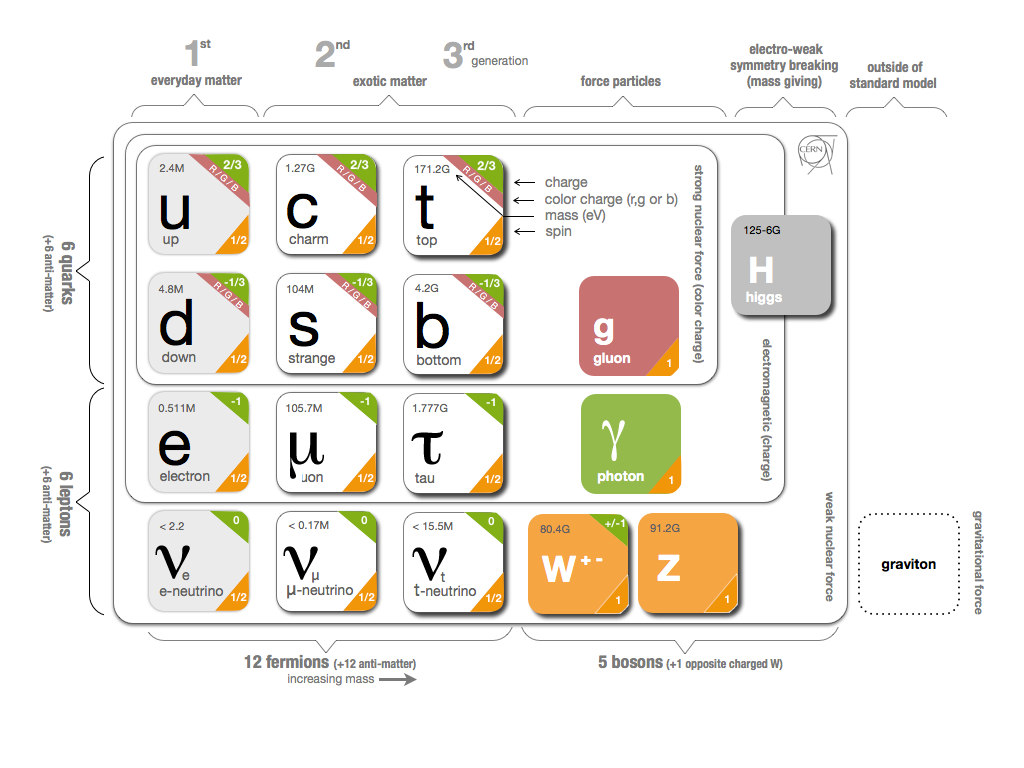
\includegraphics[width=1.15\linewidth]{Images/Part_1/SMinfographic_image.png}
\end{figure}

\subsection{Frodo be chillin} \label{sec:frodoNchill}
Not a lot happens

\subsection{Gandalf Commth} \label{sec:bitchImGandalf}
Some weird shit happens
Here's a figure on the side! Use Hspace and Vspace to fineadjust.


\chapter{The Two Towers} \label{ch:towers}
In \autoref{ch:fellowship} we see that pippin is pimpin.
The first chapter has the label 'ch:fellowship'.
Using ref gives: \ref{ch:fellowship}. Using autoref gives: \autoref{ch:fellowship}.
\marginnote{
    \hspace*{-0.5cm}
    \vspace*{0.5cm}
    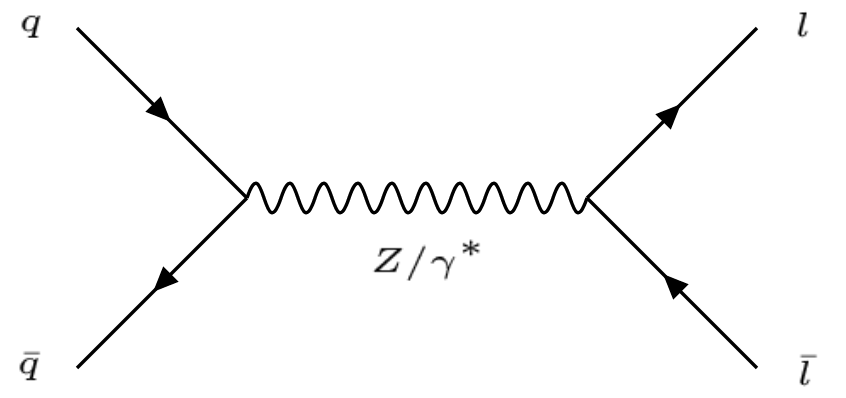
\includegraphics[width=1.6\marginparwidth]{Images/Part_1/MainDecayPath.png}
    \captionof{figure}{Feynman diagram for the $q\bar{q} \rightarrow Z/\gamma^* \rightarrow l\bar{l}$ decay where $\gamma^*$ is a virtual photon}
    \label{fig:MainDecay}
}

\subsection{Feynman diagrams} \label{sec:Feynman}
We are not only interested in the probability of collision, but also how particles in that collision decays
and what they decay to after an interaction.
This requires some theoretical calculation. Fermi's Golden rule describes the probability of some initial particle (\textit{i}) decaying
into a specific final mode \textit{f} and is given by \citep{schwartz:2006}:
\begin{ceqn}\begin{align} \label{eq:adamisgay}
  \centering
  \Gamma_{i \rightarrow f} \sim |M_{i \rightarrow f}|^2 \delta(E_f-E_i)
\end{align}\end{ceqn}
\autoref{eq:adamisgay} is an equation.

\chapter{The Return of the King} \label{ch:king}
The best one \\

An acronym the first time it is used: \ac{CERN}.\\
An acronym the post-first time: \ac{CERN}